\chapter{Projekt aplikacji}
W rozdziale tym zawarte są informacje o architekturze projektowanego systemu. Jego złożona budowa rozłożona została na części bardziej elementarne w celu przedstawienia istoty rozwiązania problemu jaki stawia sobie niniejsza praca.
\section{Architektura}
Architektura aplikacji składa się z części mobilnej oraz czterech serwisów, z czego każdy występuje jako autonomiczna aplikacja z którą porozumiewanie odbywa się za pomocą protokołu HTTP. Warstwa prezentacyjna, porozumiewając się z pozostałymi serwisami zapewnia użytkownikowi płynną interakcję z systemem. Dzięki takiej strukturze każda składowa część aplikacji może być niezależnie zarządzana. W sytuacji w której, pojedyncza usługa jest wyłączona, sama aplikacja może dalej działać, brak jej będzie jedynie funkcjonalności niedostępnego aktualnie serwisu.\\
Takie podejście można określić mianem zorientowanym na usługi. Oznacza to, że przy tworzeniu systemu, spory nacisk kładziony jest na definiowanie rozdzielnych usług. Mają one za zadanie spełniać określone wymagania użytkownika. Takie usługi są elementami oprogramowania zdolnymi do niezależnego funkcjonowania. Udostępniają realizowane funkcje poprzez zdefiniowany interfejs.
\subsection{Hypertext Transfer Protocol}
HTTP, czyli ``Protokół Przesyłania Danych Hipertekstowych to protokół warstwy aplikacji, odpowiedzialny za transmisję dokumentów hipermedialnych, jak np. HTML. Został stworzony do komunikacji pomiędzy przeglądarkami, a serwerami webowymi, ale może być używany również w innych celach. HTTP opiera się na klasycznym modelu klient-serwer, gdzie klient inicjuje połączenie poprzez wysłanie żądania, następnie czeka na odpowiedź. HTTP jest protokołem bezstanowym, co oznacza, że serwer nie przechowuje żadnych danych (stanów) pomiędzy obydwoma żądaniami. (...)``~~\cite{http}


\begin{figure}[H]
	\centering
	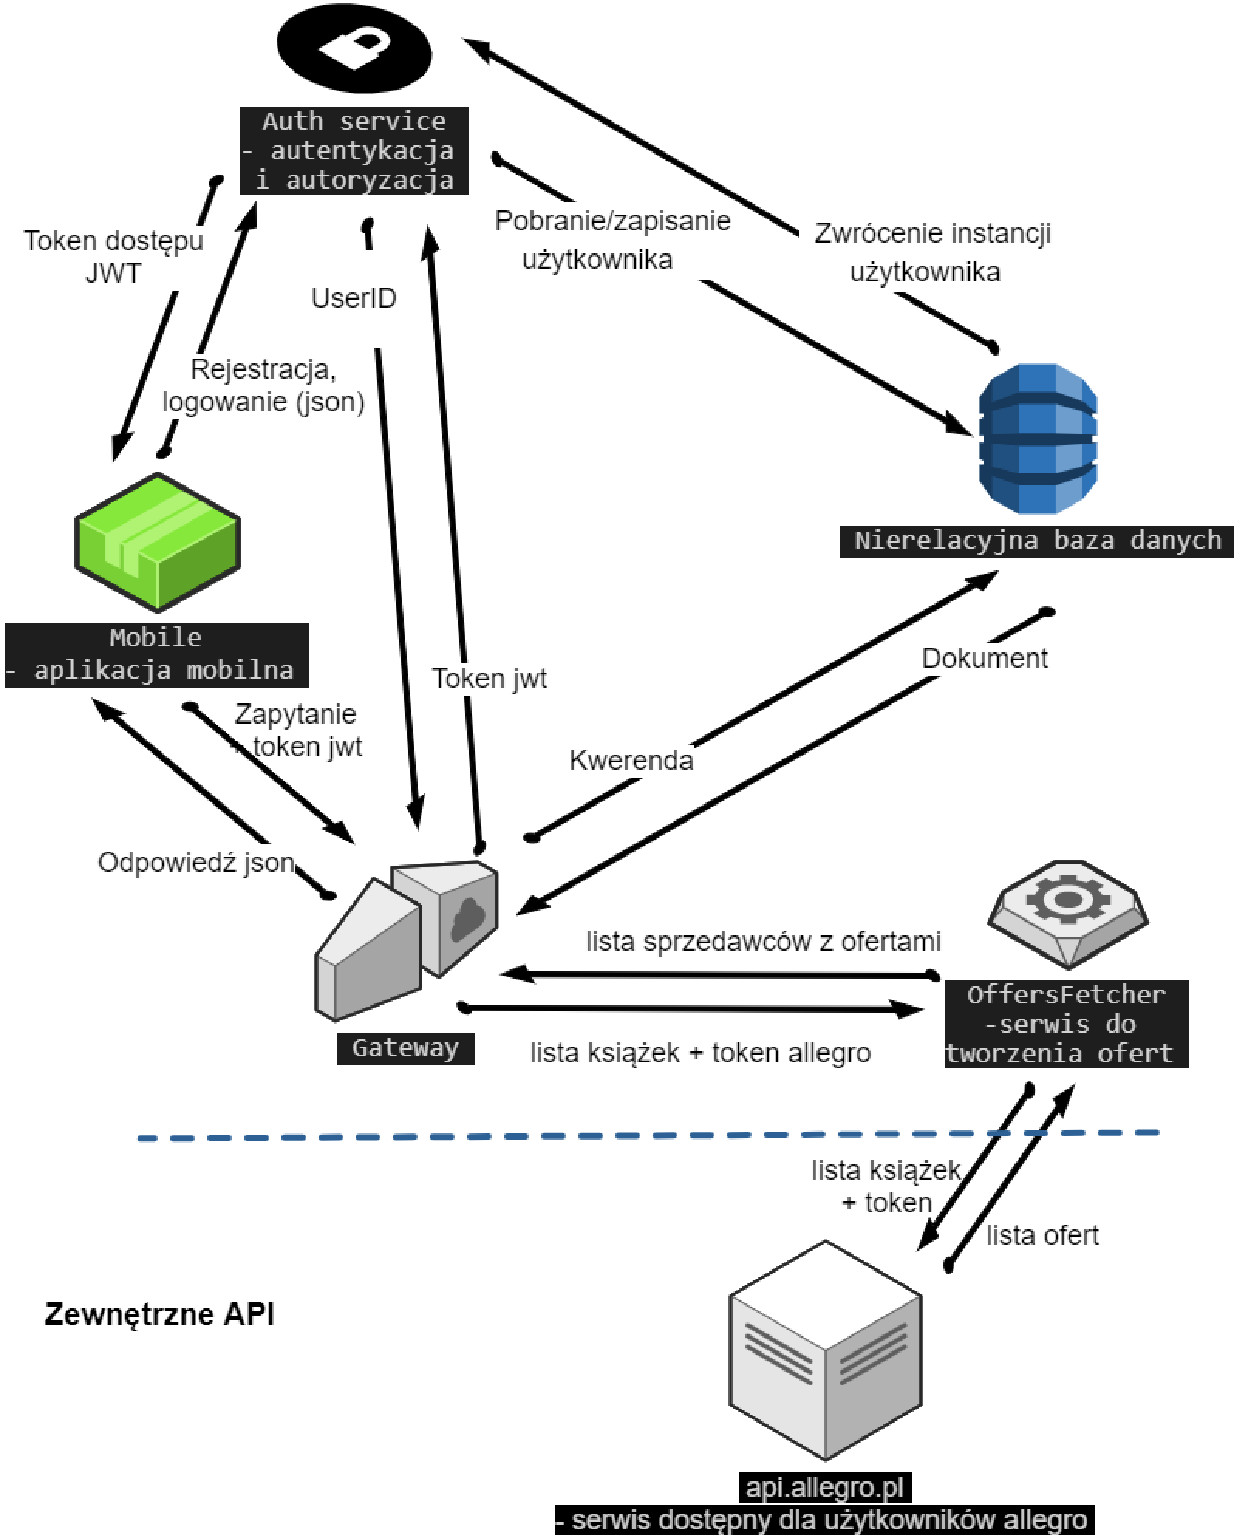
\includegraphics[width=\linewidth]{architecture_overview.pdf}
	\caption{\centering Struktura systemu}
	\caption*{\centering Źródło: {Opracowanie własne z użyciem narzędzia \url{https://www.draw.io/}}}
\end{figure}

\section{Auth service}
Auth service dba o zachowanie bezpieczeństwa w całym systemie.
Poprzez ekstrakcję funkcjonalności związanej z tworzeniem kont, logowaniem oraz zarządzaniem dostępem do pozostałych sektorów, dostarcza możliwość autentykacji i autoryzacji użytkownika pragnącego korzystać z aplikacji.
Informacje o kontach użytkowników przechowywane są w bazie danych, do której dostęp uzyskać można tylko za pomocą wygenerowanego przez nią, wewnętrznego klucza. Same hasła użytkowników są przechowywane w postaci ciągu znaków powstałego po zastosowanniu do wejściowego napisu funkcji hashującej, czyli algorytmu szyfrującego jednostronnie.

W celu swobodnego użytkowania aplikacji należy uzyskać JWT(\texttt{JSON Web Token}). Aby pozyskać token należy się zarejestrować lub zalogować w aplikacji mobilnej. Zapytanie utworzone w ten sposób zostanie wysłane do Auth service. W odpowiedzi na nie, przesłany zostanie wyżej wymieniony klucz dostępowy.

\subsection{JSON Web Token}

JSON Web Token to otwarty standard, który definiuje kompaktowy i samodzielny sposób na bezpieczny transfer danych. Poszczególna instancja składa się z trzech części oddzielonych kropkami w bezpośrednim formacie xx..x.y..yy.zz..z, gdzie poszczególne człony reprezentują:~\cite{jwt}
\begin{enumerate}%[1)]
	\item Header - nagłówek, zawierający dwie informacje:
		\begin{itemize}
			\item typ tokenu, w tym przypadku "JWT"
			\item rodzaj algorytmu szyfrującego(n.p. HMAC, SHA256 lub RSA)
		\end{itemize}

	\item Payload - lista wyrażeń opisujących szyfrowaną informację, w przypadku instancji użytkownika - może to być jego login, czy email
	
	\item Signature - podpis stworzony poprzez zaszyfrowanie podanym w nagłówku algorytmem szyfrującym ciągu składającego się kolejno z:
	\begin{itemize}
		\item zakodowanego za pomocą Base64 (specjalnego kodowania transportowego) nagłówka i listy wyrażeń
		\item sekretu, czyli klucza unikalnego dla konkretnych danych
	\end{itemize}
	\end{enumerate}

	\begin{figure}[H]
		\centering
		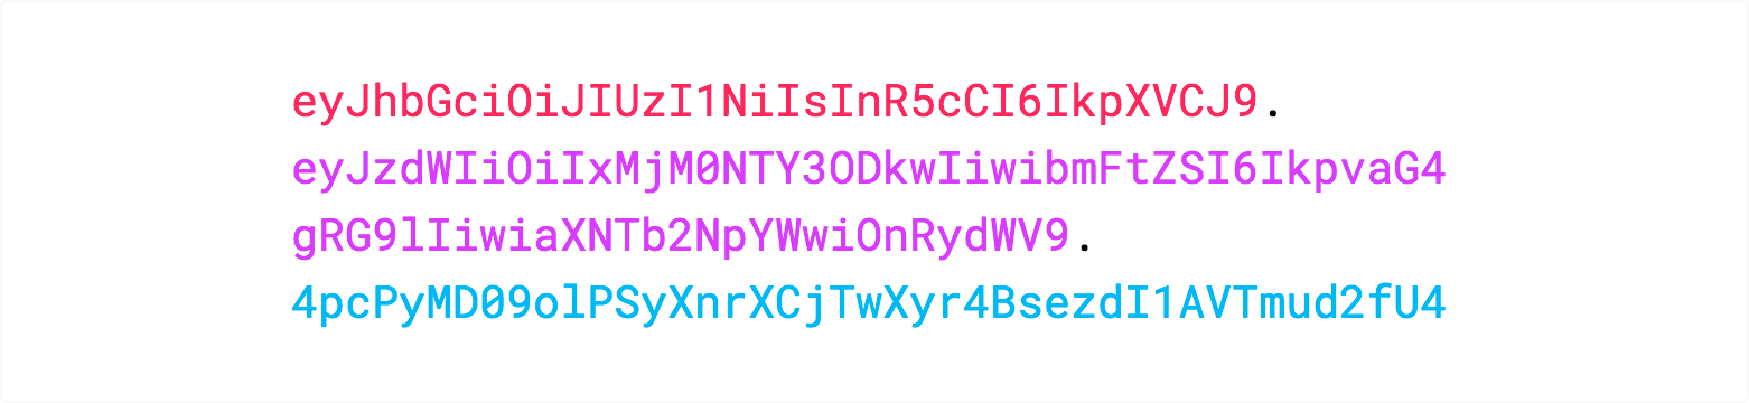
\includegraphics[width=\linewidth]{json-token.pdf}
		\caption{\centering Przykładowy token jwt}
		\caption*{\centering Źródło: \url{https://jwt.io/introduction/}}
	\end{figure}

\subsection{Autoryzacja, a autentykacja}

Warto implicite rozróżnić dwa bardzo ważne pojęcia związane z bezpieczeństwem aplikacji.

\textbf{Autentykacja}, często też rozważana w dwóch kolejnych częściach składowych - jako identyfikacja i uwierzytelnienie. Polega na potwierdzeniu tożsamości, to znaczy określeniu, czy podmiot procesu jest tym za kogo się podaje. Na przypadku logowania: strona ufająca otrzymuje od użytkownika login i hasło. Na tej podstawie stwierdza, czy użytkownik może być pozytywnie zweryfikowany.

\textbf{Autoryzacja} to potwierdzenie, czy dany użytkownik jest uprawniony do skorzystania z konkretnego zasobu. Na tym etapie autentykacja została ewaluowana pozytywnie. Nie oznacza to jednak, że dany podmiot posiada dostęp w żądanym zakresie. 

\section{Gateway}
Gateway to serwis zbudowany według podejścia zwanego \texttt{wzorcem bramy interfejsu API}~\cite{richardson2018api}. Jest to element znajdujący się pomiędzy klientem a rozproszonymi usługami. Dzięki temu w prosty sposób można kontrolować wszelkie zapytania skierowane do poszczególnych serwisów.
Jest to więc centralny punkt systemu, który ma na celu uproszczenie komunikacji warstwy prezentacyjnej z poszczególnymi usługami. Każde zapytanie wysłane do bramy zostaje zweryfikowane pod względem bezpieczeństwa. Następnie w zależności od potrzeb, modyfikowane lub bezpośrednio przesyłane dalej.
\begin{figure}[H]
	\centering
	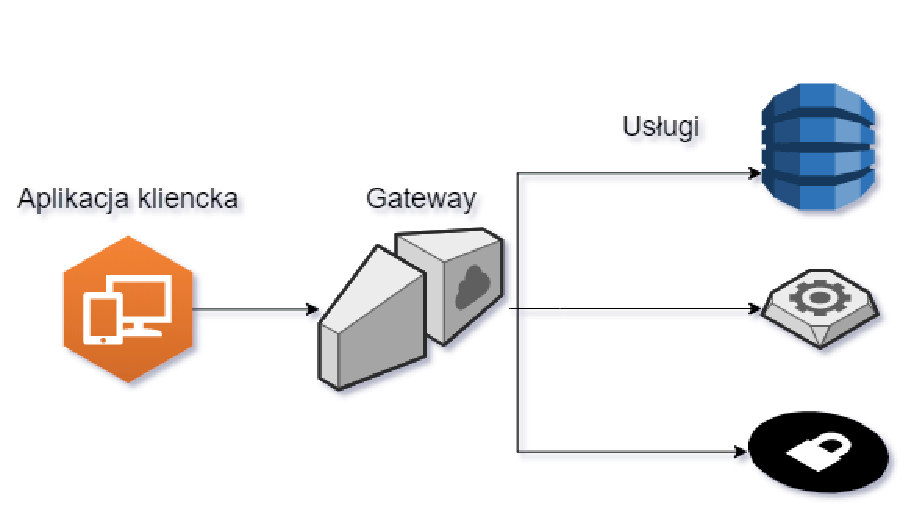
\includegraphics[width=\linewidth]{gateway.pdf}
	\caption{\centering Gateway - schemat}
	\caption*{\centering Źródło: {Opracowanie własne z użyciem narzędzia \url{https://www.draw.io/}}}
\end{figure}

\section{OffersFetcher}
OffersFetcher to główna jednostka licząca w systemie. Usługa ta otrzymuje żądanie z listą książek oraz token dostępowy do REST API portalu Allegro.pl (2.5).
Dla każdej książki wykonywane jest odpowiednio zmodyfikowane zapytanie, którego rezultat jest przetwarzany i odkładany do kolekcji, aby na koniec zostać wkomponowanym w wynikowy rezultat. Analizowane są wszystkie, obecnie dostępne w czasie rzeczywistym oferty sprzedaży w serwisie Allegro.pl. Dane otrzymane w ten sposób są przetwarzane i grupowane po unikalnym identyfikatorze sprzedawcy. Serwis zwraca odpowiedź w postaci listy zbiorów przedmiotów, które wpisują się w pozyzcje otrzymane w zapytaniu. W celu optymalizacji czasu w którym przygotowana zostaje odpowiedź, pobieranie danych oraz obliczenia wykonywane są asynchronicznie, co znacznie przyspiesza proces generowania wyników.
\begin{figure}[H]
	\centering
	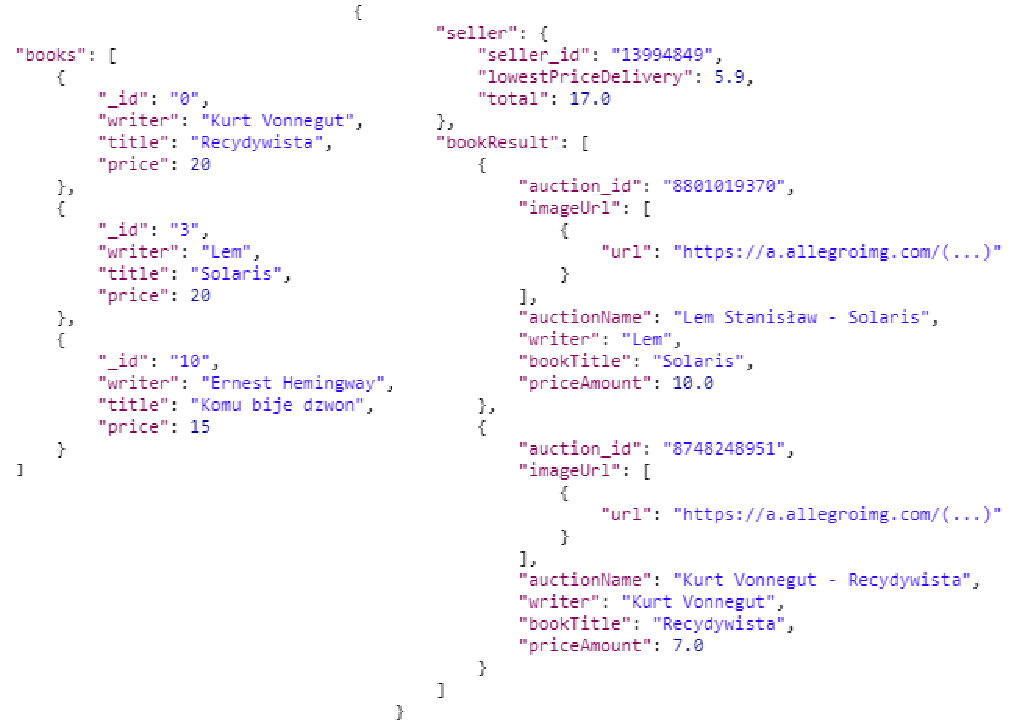
\includegraphics[width=\linewidth]{booksToOffers.pdf}
	\caption{\centering Poszukiwane książki i bazująca na nich przykładowa oferta}
	\caption*{\centering Źródło: {Opracowanie własne}}
\end{figure}

\section{Zewnętrzne API}

Źródłem danych dla ofert tworzonych w serwisie OffersFetcher (2.4)
jest Allegro REST API udostępnione przez Allegro.pl, czyli platformę transakcyjną on-line przedsiębiorstwa Allegro.pl. Portal ten umożliwa użytkownikom wystawianie na sprzedaż posiadanych przez nich przedmiotów oraz na korzystanie z ofert innych sprzedawców.  Początkowo innym, alternatywnym rozwiązaniem miało być pobieranie całych stron HTML po uprzednim sfabrykowaniu URI, tak aby pasowało do zadanej pozycji. Następnie taki plik tekstowy miałby być przeszukiwany wyrażeniami regularnymi w celu ekstrakcji szukanych informacji. Z racji jednak na dość niestabilny i zasobochłonny chrakter, wybrano korzystanie\\z gotowego źródła danych w postaci dostarczonego API.\newline
``Allegro REST API działa w oparciu o protokół HTTP (...) Autoryzacja realizowana jest w standardzie OAuth2.``~\cite{allegroApi}

\subsection{REST API}
(\textbf{RE}presentational \textbf{S}tate \textbf{T}ransfer) to styl architektury oprogramowania w którym dane i funkcjonalności są odzwierciedlone poprzez Ujednolicone Identyfikatory Zasobów\\(w skrócie URI). Termin ten został stworzony przez Roya Fieldinga w 2000 roku. Dostęp uzyskiwany jest poprzez proste i jasno zdefiniowane operacje.  Istnieje pięc obowiązkowych ograniczeń, które dokładnie definiują charakter tego podejścia:
\begin{itemize}
	\item bezstanowość - każde zapytanie do serwera powinno zawierać wszystkie informacje potrzebne do jego zrozumienia.
	\item użycie buforownia podręcznego - jeżeli dane są lokalnie przechowywane, należy\\o tym bezpośrednio poinformować.
	\item system warstwowy - istnieje możliwość użycia wielu komponentów do poszczególnych funkcjolności, które razem stanowią jedno API. Klient przeważnie nie jest w stanie określić, czy jego połączenie jest realizowane z serwerem końcowym czy którymś\\z pośredników.
	\item rozdział klienta od serwera - obie części powinno się być w stanie rozwijać osobno\\i niezależnie. Klient powinien jedynie znać URI, które może odpytywać.
	\item ujednolicony interfejs - należy deterministycznie zdefiniować i nie zmieniać adresów pod którymi dostępne będą zasoby. 
\end{itemize}~\cite{fielding}

\section{Baza danych}
Warstwa persystencyjna jako osobny i niezależny serwis ma zadanie przetrzymywać dane użytkowników aplikacji. Jest to ogromnie ważny element systemu, którego działanie niezbędne jest na przykład dla Auth service (2.2). Wykorzystuje on go ze względu na posiadane informacje, które używane są w celu autoryzacji i autentykacji.
Oprócz danych dostępowych, dla każdego klienta przechowywane są również zbiory książek - posiadanych i poszukiwanych.\newline
Istniejące aktualnie, złożone bazy danych można podzielić ze wględu na struktury organizacji danych jakie stosują do ich przechowywania. Są to kolejno relacyjne, obiektowe, relacyjno-obiektowe, strumieniowe, temporalne, nierelacyjne (NoSQL).

\subsection{Bazy relacyjne}
Najczęściej spotykane są nadal bazy relacyjne, gdzie dane występują pod postacią powiązanych wzajemnie ze sobą tabel. Stosują one wewnętrzne języki programowania(wykorzystujące zwykle język SQL), służące do wykonywania zaawansowanych operacji.
\begin{figure}[H]
	\centering
	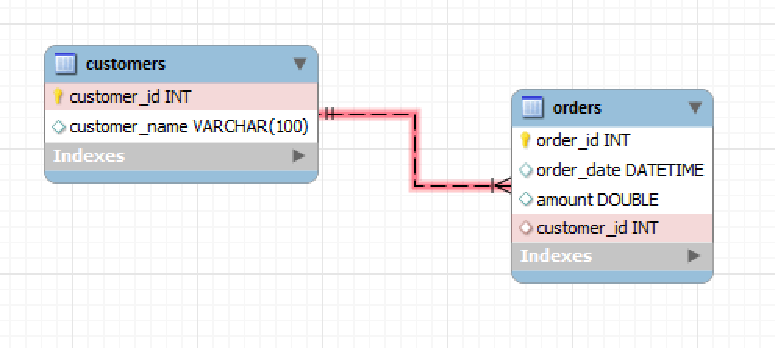
\includegraphics[width=\linewidth]{relations.pdf}
	\caption{\centering Przykład dwóch tabel i relacji pomiędzy nimi}
	\caption*{\centering Źródło: \url{code.tutsplus.com}}
\end{figure}

\subsection{Bazy nierelacyjne}
Sporą popularność zyskują ostatnio bazy nierelacyjne, czyli takie, które nie posiadają tabel ani relacji. W związku z tym przeważnie nie wykorzystują również języka SQL i to z stąd wzięła się ich nazwa - NoSQL (Not Only SQL database). Nie jest najczęściej też wymagane, aby struktura danych była jednorodna.
\begin{figure}[H]
	\centering
	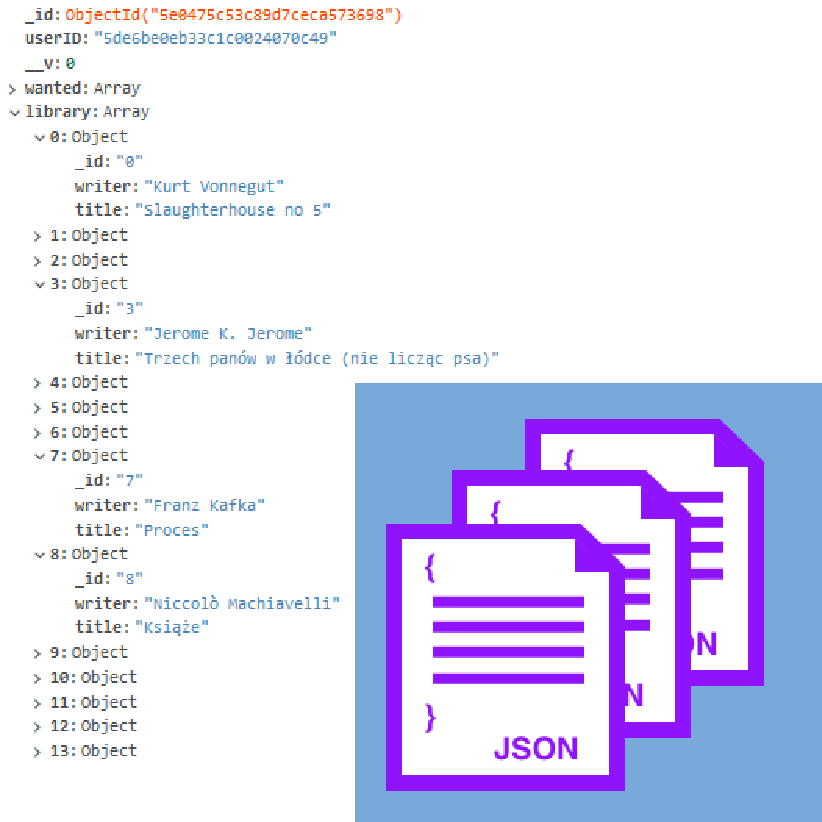
\includegraphics[width=\linewidth]{nosql.pdf}
	\caption{\centering Przykład obiektu json w bazie NoSQL przechowującej dane jako dokumenty}
	\caption*{\centering Źródło: {Opracowanie własne z użyciem fragmentu grafiki ze strony \url{https://medium.com}}}
\end{figure}

\subsection{Porównanie}
Przewagę relacyjnych baz danych można upatrywać w istotnie ugruntowanym interfejsie, stosunkowo łatwym utrzymaniu i tym, że w związku z wybitną popularnością, zestandaryzowany język zapytań daje programistom gotowy, ogólny pogląd na dowolną relacyjną bazę danych z którą przyjdzie im pracować.
Jednakże bazy typu NoSQL reprezentuje łatwa skalowalność oraz bardzo szeroki wybór modeli danych. Są one też szybsze, bardziej wydajne a ponadto daleko bardziej elastyczne. Nie wymagają być administrowanymi i obecnie rozwijają się coraz prężniej.~\cite{database}

\section{Aplikacja mobilna}
Komponent w którym spotykają się wszystkie części składowe systemu. Podejście mobilne zostało wybrane ponieważ rynek związany z urządzeniami mobilnymi to obecnie najszybciej rozwijająca się gałąź przemysłu IT~\cite{mobile}. Dzięki temu produkt może potencjalnie trafić do szerszego grona odbiorców, zwłaszcza, że nie wymaga od użytkownika skomplikowanych czynności i można z niego korzystać na przykład w komunikacji miejskiej.

\subsection{Przystępność produktu}
Tworząc oprogramowanie, którego ma używać człowiek, warto zadbać o to, aby\\w pierwszej kolejności było ono dla niego ułatwieniem, które z chęcią wykorzysta.
\subsubsection{Podstawowe cechy przyjaznej użytkownikowi aplikacji}
 Ze względu na ograniczone medium jakim jest urządzenie mobilne, ważnym jest aby dostarczyć rozwiązanie, którego odbiorca chciałby używać. Warto więc zastanowić się nad określeniem aspektów, które składają się na przyjazną użytkownikowi formę.\newline
 ``Podstawowe atrybuty opisujące użyteczność aplikacji zostały zidentyfikowane w klasycznej pracy Nielsena~\cite{usability}: 
 \begin{itemize}
	 \item efektywność (efficiency) – łatwość uzyskania celu,
	 \item satysfakcja (satisfaction) – brak dyskomfortu, pozytywne nastawienie do
	 produktu
	 \item przyswajalność (learnability) – łatwość nauczenia się zasad działania w celu szybkiego rozpoczęcia pracy,
	 \item zapamiętywalność (memorability) – łatwość powrotu do pracy z systemem
	 po przerwie
	 \item bezbłędność (faultlessness) – ograniczenie liczby popełnianych błędów oraz zdolność do wznowienia działania po awarii
 \end{itemize}
 Najłatwiej zmierzyć efektywność, która w wielu sytuacjach może zostać
 wyrażona jako czas potrzebny do wykonania określonego zadania. Pozostałe
 atrybuty są znacznie bardziej abstrakcyjne, a wśród nich największy ładunek
 subiektywnych emocji z pewnością niesie satysfakcja użytkownika.``~\cite{mobile}

 \subsubsection{Funkcjonalności implementujące atrybuty zidentyfikowane przez Nielsena}
 Tworzenie oprogramowania na urządzenia przenośne wymaga więc dokładnego zaplanowania interfejsu graficznego, który będzie nie tylko przyjazny wizualnie, ale i funkcjonalny. Zakłada się, że zaprezentuje odbiorcy możliwe funkcjonalności w sposób oczywisty i jednoznaczny. Powinien on więc płynnie i możliwie szybko odpowiadać na akcje użytkownika. Ze względu na odpowiednio mniejszą moc obliczeniową, należy zadbać o użycie właściwych elementów sterujących oraz zadbać o wydajne renderowanie. W ten sposób można uniknąć przechowywania niepotrzebnych referencji do wykorzystanych wcześniej obiektów oraz zwrócić uwagę na to, aby obliczenia wykonywane przez urządzenie nie były nazbyt skomplikowane. W trosce właśnie o to, zaawansowana logika licząca została wyekstraktowana do osobnego serwisu (3.4). Poprzez przechowywanie informacji w bazie danych, gwarantujemy, że po ponownym włączeniu aplikacji, nawet po wymuszonym zamknięciu - użytkownik nie straci swoich zmian.